\documentclass[12pt]{article}

% Basic packages
\usepackage[utf8]{inputenc}
\usepackage{csquotes}
\usepackage{geometry}
\geometry{a4paper, margin=1in}
\usepackage{graphicx}  % Include the graphicx package to add figures
\usepackage{caption}   % Enhanced caption handling
\usepackage{postnotes}
\postnotesetup{
  format={\normalsize \raggedright},  % Set the endnotes text to 12pt and left-align
  listenv=none,  % Disable the list environment to align notes to the left
  heading=\mycustomheading  % Custom heading to eliminate space after
}

% Custom heading command to remove space after
\newcommand{\mycustomheading}{
  \section*{Notes}
  \vspace{-\baselineskip} % Remove the space after the heading
}

% Title setup
\usepackage{titlesec}

% Aligning all section headings to the left
\titleformat{\section}
  {\normalfont\normalsize\bfseries}{\thesection}{1em}{}
\titleformat{\subsection}
  {\normalfont\normalsize\bfseries}{\thesubsection}{1em}{}
\titleformat{\subsubsection}
  {\normalfont\normalsize\bfseries}{\thesubsubsection}{1em}{}

% Font selection
\usepackage[T1]{fontenc}
\usepackage{times}

% Hyperlink setup
\usepackage[colorlinks=true, allcolors=blue]{hyperref}

% BibLaTeX setup for Harvard style with full first names
\usepackage[backend=biber, style=authoryear, maxcitenames=2, giveninits=false, natbib=true, uniquename=full]{biblatex}
\addbibresource{references.bib} % Specify the bibliography file
% Redefine the bibliography heading to remove space after
\defbibheading{bibliography}[\bibname]{%
  \section*{References}
  \vspace{-\baselineskip}
}

% Redefine the abstract environment to adjust spacing
\renewenvironment{abstract}
  {\begin{flushleft}
   \bfseries \abstractname\vspace{-1em} % Adjust the vertical space after the heading
   \end{flushleft}
   \list{}{%
     \setlength{\leftmargin}{0mm}%
     \setlength{\rightmargin}{\leftmargin}%
   }%
   \item\relax}
  {\endlist}


% Define command for keywords
\newcommand{\keywords}[1]{%
    \noindent\textbf{Keywords:} #1
}

%------------------------------------------------------------
% Title setup
%------------------------------------------------------------
% Redefine \maketitle to align the title left and make it 12pt
\makeatletter
\renewcommand{\maketitle}{
  \begin{flushleft} % Align left
    \textbf{\@title} % Title in 12pt, bold
    \vspace{1em} % Space after the title
  \end{flushleft}
}
\makeatother
\title{Test v0.1.29}
% \author{Kynan Stewart Hughes\\ \texttt{kynan.s.hughes@student.uts.edu.au}}
\date{}
%------------------------------------------------------------

\begin{document}

\maketitle

\begin{abstract}
Your abstract text goes here.
\end{abstract}

% Insert keywords
\keywords{Keyword 1, Keyword 2, Keyword 3, Keyword 4, Keyword 5, Keyword 6}

\section*{Introduction}
The introduction text goes here. You can cite sources using \textcite{RindCmplxtyAndClmt1999} for textual citations, or \parencite{RindCmplxtyAndClmt1999} for parenthetical citations \parencite[see][p.35]{Bell_PhilosophyAtTheEdgeOfChaos_2006}.

\section*{Methodology}
The methodology text goes here\postnote{
    This is a postnote.
}.

% Adding a figure
\begin{figure}[htb]
    \centering
    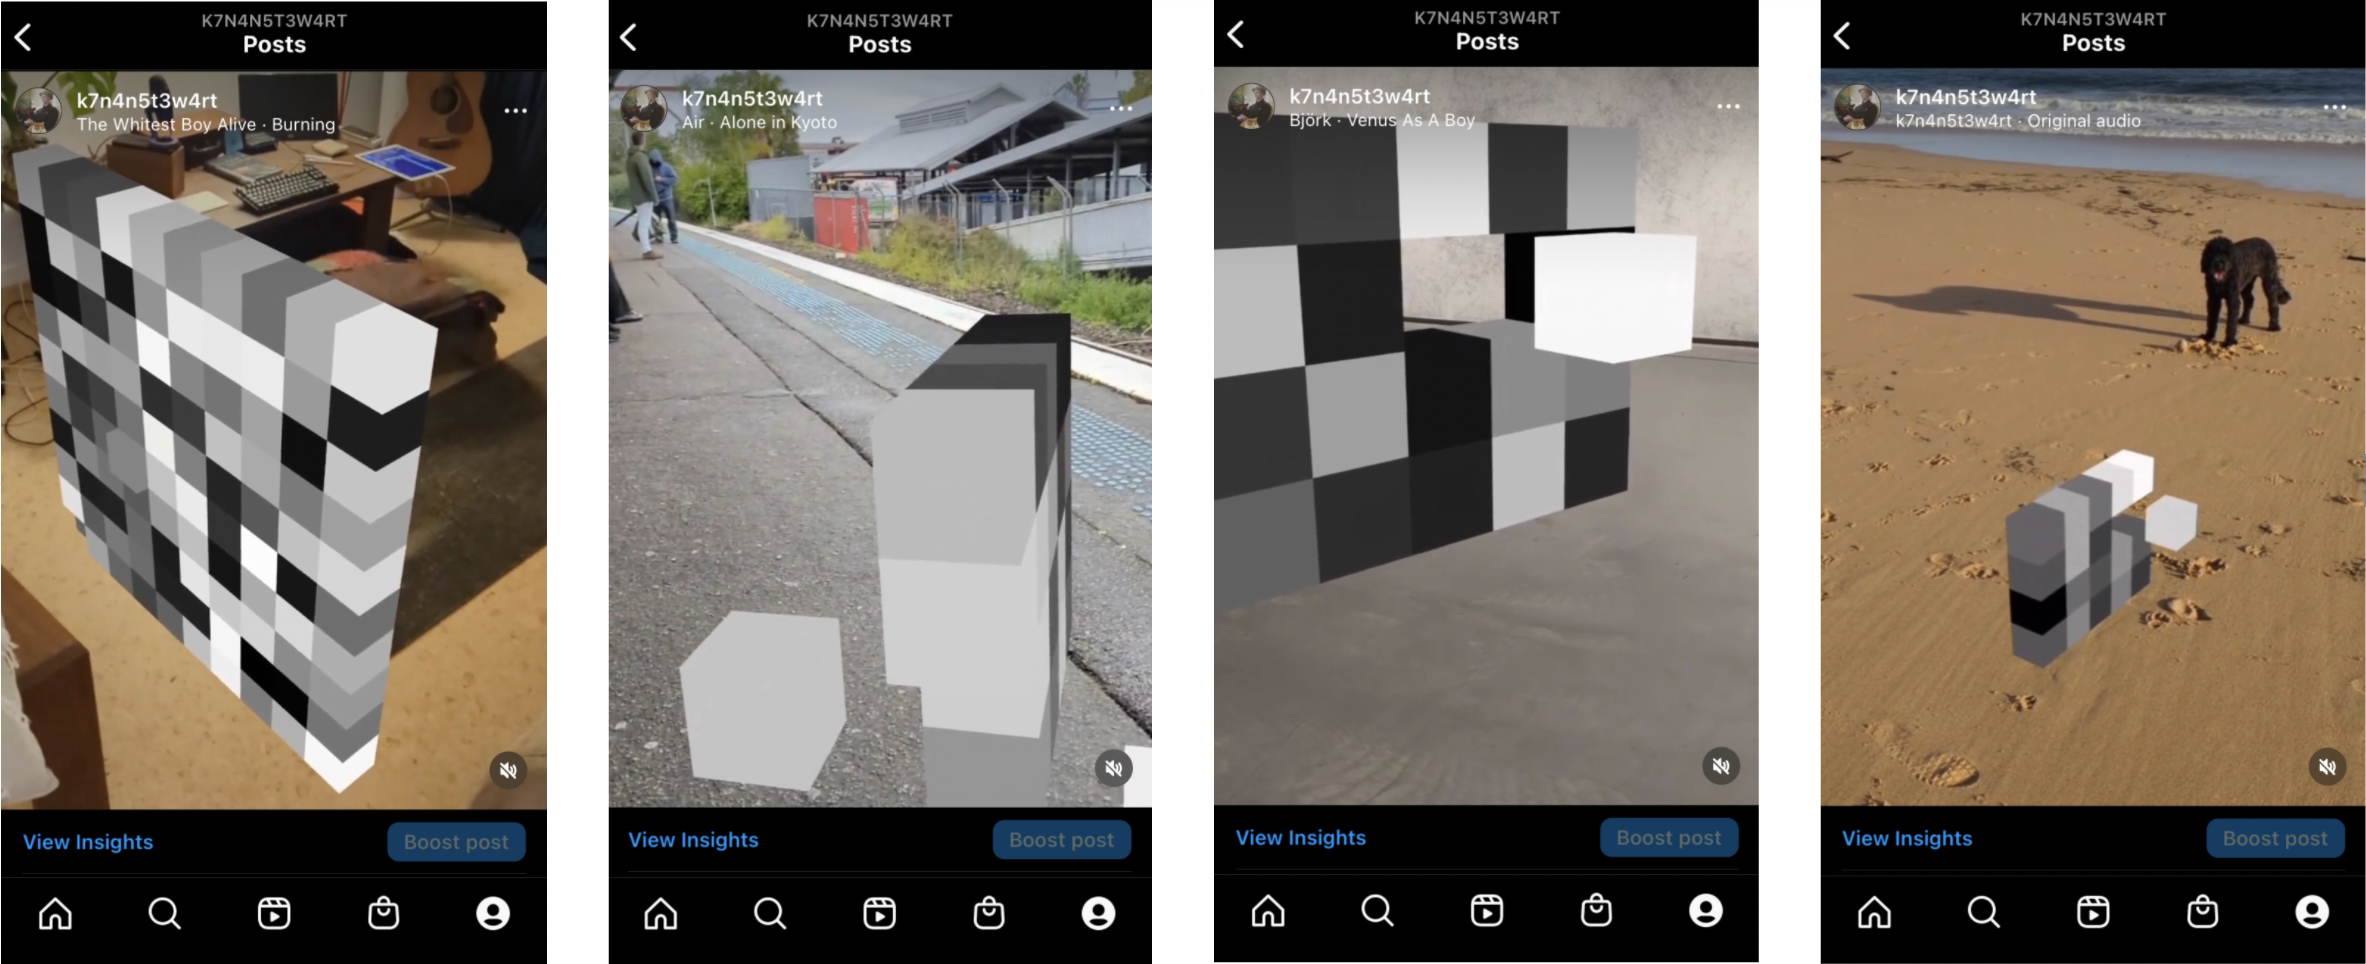
\includegraphics[width=0.8\textwidth]{figures/algorithms-1.png}  % Adjust the path and filename to your image
    \caption{This is an example caption.}
    \label{fig:exampleFigure}
  \end{figure}

\section*{Results}
The results text goes here.

\section*{Discussion}
The discussion text goes here.

\section*{Conclusion}
The conclusion text goes here. Testy...

% Printing endnotes
\printpostnotes

\printbibliography[heading=bibliography]


\end{document}